\documentclass[11pt]{article}
\usepackage[margin=1in]{geometry}
\usepackage{booktabs}
\usepackage{graphicx}
\usepackage{hyperref}
\title{ActuarialBench: Reproducible Benchmark of Frontier LLM Reliability in Actuarial Science}
\author{Amine Manai}
\date{\today}
\begin{document}
\maketitle
\begin{abstract}
ActuarialBench is a reproducible protocol for evaluating black-box language-model endpoints on objectively gradable actuarial tasks. The benchmark separates mathematical correctness, executable code correctness, validation-defect detection, schema reliability, latency, and cost. Results are paired by task and repetition and reported with uncertainty; no global superiority claim is made without statistical support.
\end{abstract}
\section{Introduction}
Actuarial model risk depends on whether a system applies assumptions, formulas, and validation controls correctly under incomplete information. This study evaluates those observable behaviors rather than subjective fluency.
\section{Research Questions}
The protocol asks which routes are accurate, reliable, calibrated, and efficient across actuarial domains, and which failure categories explain observed differences.
\section{Benchmark Design}
The initial vertical slice contains eight deterministic tasks generated from fixed seeds. Each task stores a prompt, independently computed reference answer, tolerance, domain, and grading policy.
\section{Ground Truth and Grading}
Numerical components use analytic formulas and justified tolerances. Validation tasks use exact planted defect codes. Coding tasks use hidden cases and restricted subprocess execution. Explanations are secondary checks and do not replace primary correctness.
\section{Experimental Controls}
The manifest records task hashes, prompt hashes, seeds, routes, configuration, and Git commit. Fresh context and the same task text are used for every route. Provider failures remain separate from model failures.
\section{Statistical Methodology}
Model comparisons are paired by task and repetition. The analysis reports bootstrap intervals, paired sign-permutation tests, and Holm-adjusted p-values. Small or uncertain differences are reported as inconclusive.
\section{Results}
Generated results are included from the experiment artifacts rather than typed into the report. The overall table is generated by \texttt{generate\_report\_assets.py}.
\IfFileExists{generated/overall_table.tex}{\begin{tabular}{lrrrrrr}
\toprule
Route & Calls & Capability $n$ & All-call mean & Capability mean [95\% CI] & Exact correct & API fail \\
\midrule
claude-opus-5 & 144 & 141 & 0.858 & 0.876 [0.826, 0.922] & 116/144 & 2.1\% \\
gpt-5.6-sol & 144 & 144 & 0.845 & 0.845 [0.786, 0.899] & 119/144 & 0.0\% \\
deepseek-v4-flash & 144 & 144 & 0.630 & 0.630 [0.554, 0.708] & 89/144 & 0.0\% \\
glm-5.3 & 144 & 130 & 0.516 & 0.571 [0.488, 0.650] & 60/144 & 9.7\% \\
\bottomrule
\end{tabular}
}{}
\IfFileExists{../figures/overall_accuracy.png}{\begin{figure}[h]\centering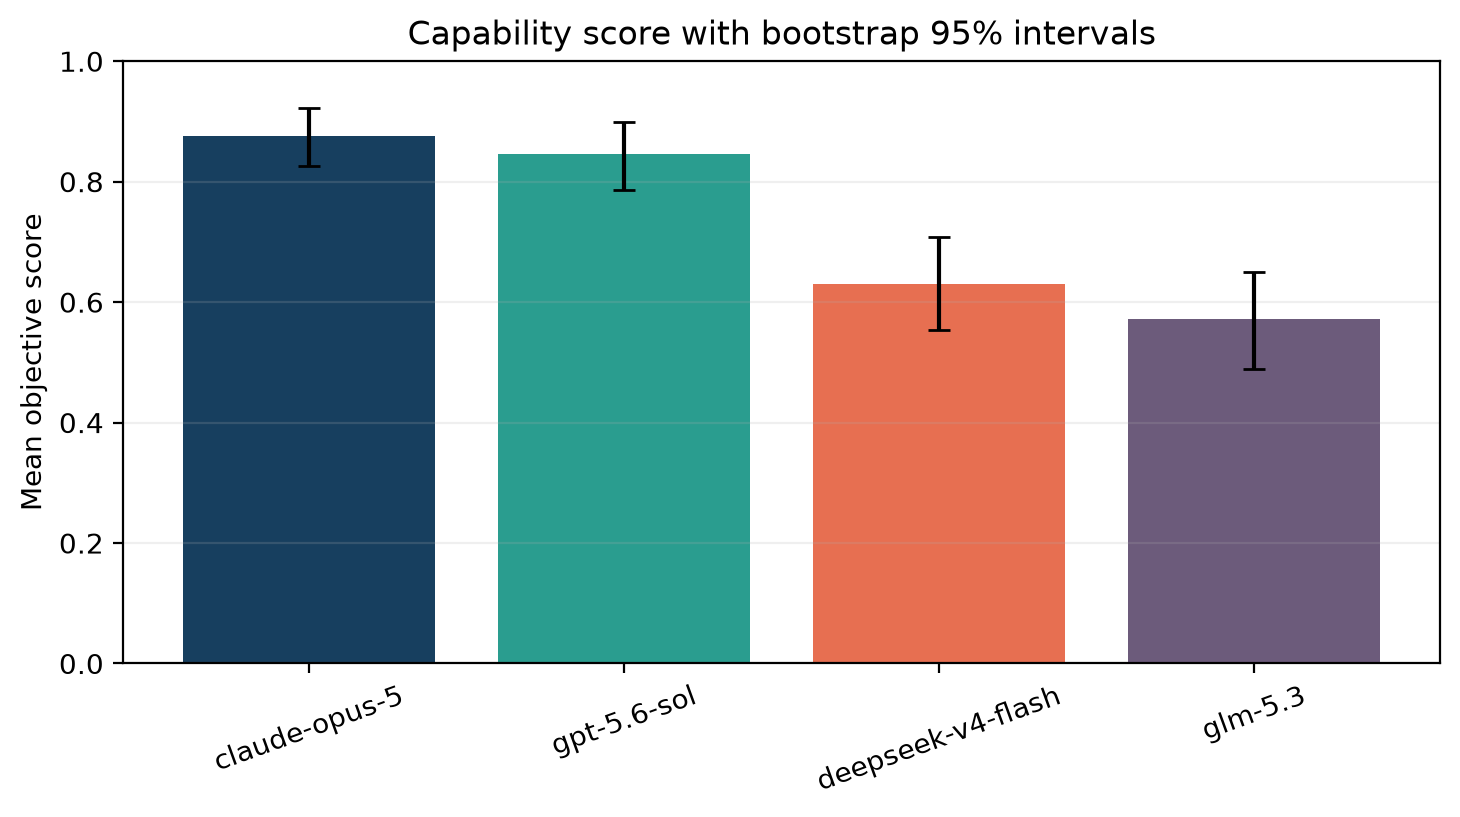
\includegraphics[width=0.85\textwidth]{../figures/overall_accuracy.png}\caption{Overall objective score with bootstrap intervals.}\end{figure}}{}
\section{Failure Analysis}
Failure tags distinguish numerical, formula, assumption, hallucination, code, schema, validation, timeout, and provider errors.
\section{Cost and Latency}
Provider-reported cost and latency are descriptive efficiency measures. Unknown pricing is retained as unknown.
\section{Limitations and Threats to Validity}
AgentRouter route identity is externally asserted rather than independently verified. The initial task bank is deliberately small, and restricted subprocess execution is not a hardened sandbox. Standard actuarial formulas may also be present in model training data; generated parameter combinations test application rather than formula novelty.
\section{Conclusion}
ActuarialBench is designed to support a defensible, uncertainty-aware comparison after the task bank and experiment manifest are frozen. It does not justify a universal model ranking from a single score.
\end{document}
